\section{Reference Model}

\begin{figure}
    \centering
    \begin{subfigure}[t]{0.3\textwidth}
        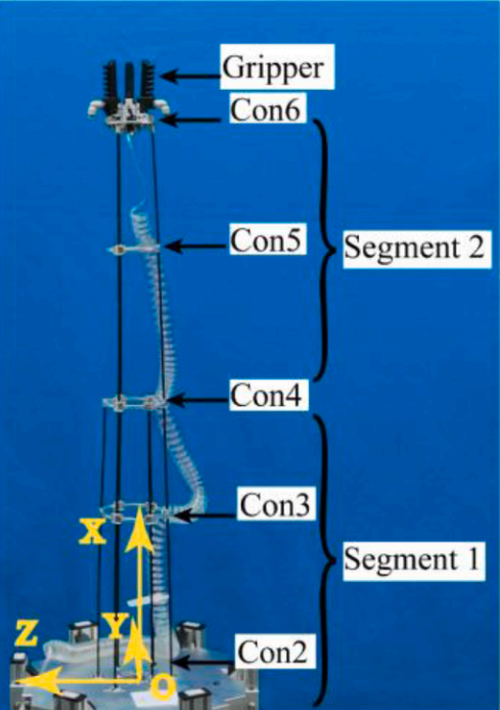
\includegraphics[width=\textwidth]{ref_robot}
        \caption{Sections and structure}
        \label{fig:ref_robot_structure}
    \end{subfigure}
    \begin{subfigure}[t]{0.3\textwidth}
        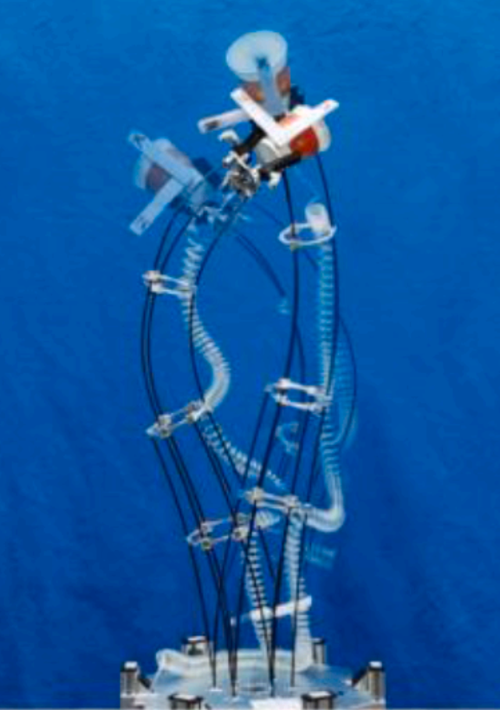
\includegraphics[width=\textwidth]{ref_robot_poses}
        \caption{Some end poses}
        \label{fig:ref_robot_poses}
    \end{subfigure}
    \caption{Reference robot structure}
    \caption*{Source: Adapted from \cite{wu2022}}
    \label{fig:ref_robot}
\end{figure}

\begin{figure}
    \centering
    \begin{subfigure}[t]{0.257\textwidth}
        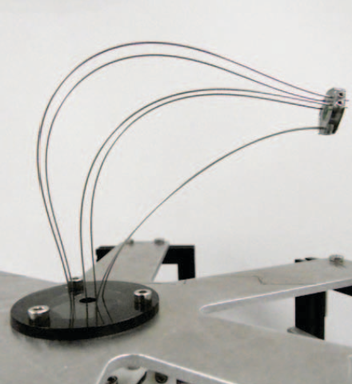
\includegraphics[width=\textwidth]{ref_robot2}
        \caption{No constraints}
        \label{fig:ref_robot2}
    \end{subfigure}
    \begin{subfigure}[t]{0.643\textwidth}
        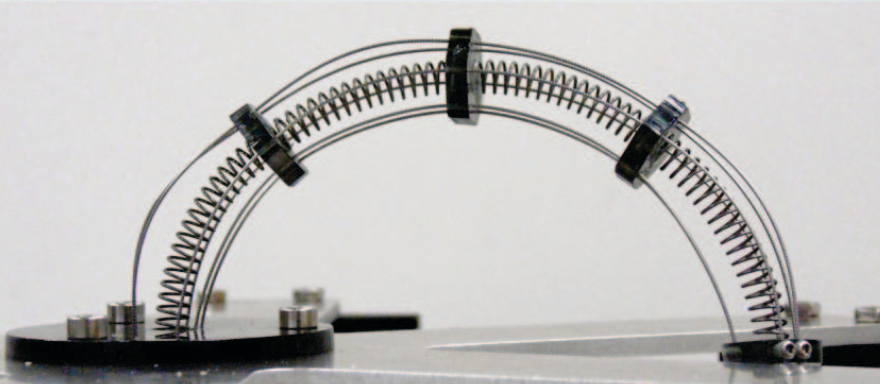
\includegraphics[width=\textwidth]{ref_robot2_cons}
        \caption{Extended range with intermediate constraints}
        \label{fig:ref_robot2_cons}
    \end{subfigure}
    \caption{Constraints and range of motion}
    \caption*{Source: Adapted from \cite{orekhov2017}}
    \label{fig:ref_robot2_constraints}
\end{figure}

\section{Rod Material}

$L \gg r$

Maximum deflection Euler-Bernoulli beam
\begin{equation}
    \delta_{max}=\frac{PL^3}{3EI}
\end{equation}

\begin{equation}
    I=\frac{\pi D^4}{64}
\end{equation}

\begin{table}[]
    \centering
    \caption{Fiberglass and AISI 302 steel properties}
    \label{tab:material-properties}
    \begin{tabular}{@{}clcc@{}}
    \toprule
    Symbol & Property                   & Fiberglass & AISI 302 \\ \midrule
    $\rho$ & Density {[}$g/cm^3${]}        & 2.6        & 8.0      \\
    $E$    & Young's Modulus {[}GPa{]}  & 85         & 187.5    \\
    $G$    & Shearing Modulus {[}GPa{]} & 36         & 70.3     \\ \bottomrule
    \end{tabular}
\end{table}


\begin{table}[]
    \centering
    \caption{Comparison between Wu \& Shi (2022) model and custom test model}
    \label{tab:comparison}
    \begin{tabular}{@{}lcc@{}}
    \toprule
    Parameter                  & \multicolumn{1}{l}{Wu \& Shi model \cite{wu2022}} & \multicolumn{1}{l}{Custom test model} \\ \midrule
    Maximum length             & $\sim860$ mm                     & $\sim450$ mm                       \\
    Minimum length             & $\sim400$ mm                     & $\sim250$ mm                        \\
    Diameters of constraints   & $[90, 80, 70, 60]$ mm               & $[55, 50, 45]$ mm                     \\
    Base constraint diameter   & 100 mm                              & 70 mm                                 \\
    Number of sections         & $2$                                 & $2$                                   \\
    Number of rods             & $6$                                 & $6$                                   \\
    Rod cross-section diameter & $3$ mm                              & $0.8$ mm                              \\
    Rod material               & Fiberglass                          & AISI 302                              \\ \bottomrule
    \end{tabular}
\end{table}

\begin{figure}
    \centering
    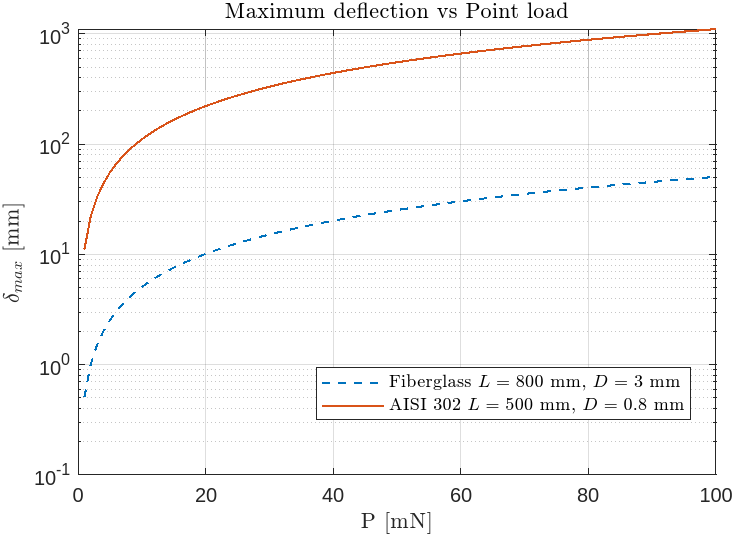
\includegraphics[width=0.8\textwidth]{force_deflection}
    \caption{Maximum deflection and point load}
    \label{fig:force_deflection}
\end{figure}

\section{Design and Dimensions}


\begin{figure}
    \centering
    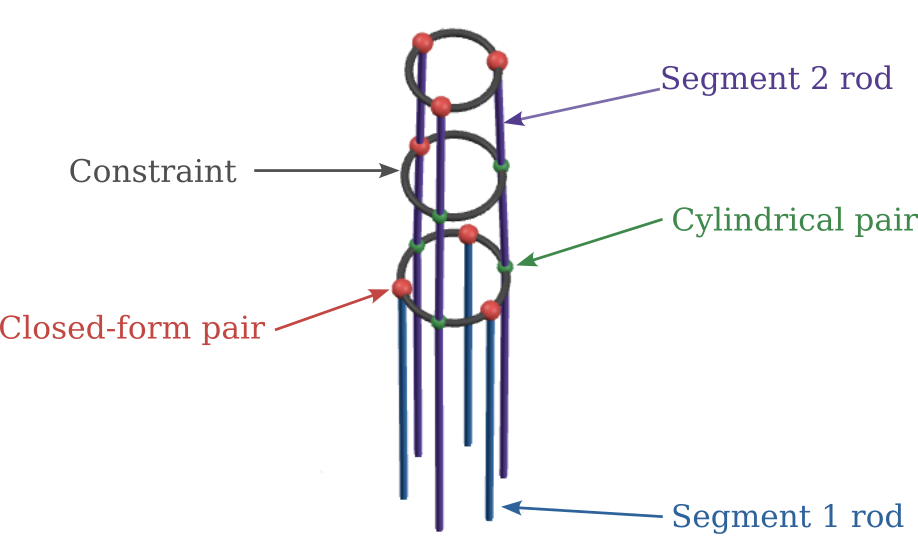
\includegraphics[width=0.7\textwidth]{rod_body_parts}
    \caption{Robot body constraints and parts}
    \label{fig:bodyparts}
\end{figure}


\begin{figure}
    \centering
    \begin{subfigure}[t]{0.2625\textwidth}
        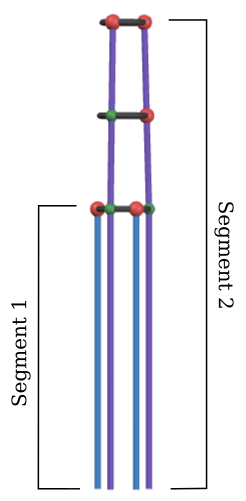
\includegraphics[width=\textwidth]{rod_body_segments}
        \caption{Left view, and robot body segments}
        \label{fig:segments}
    \end{subfigure}
    \begin{subfigure}[t]{0.4375\textwidth}
        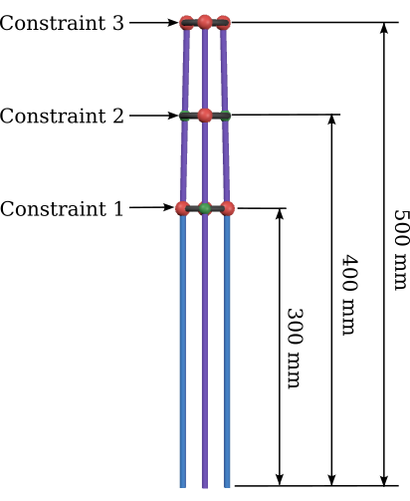
\includegraphics[width=\textwidth]{constraint_heights}
        \caption{Frontal view, and constraints heights}
        \label{fig:cons_heights}
    \end{subfigure}
    \caption{Robot body lateral views}
\end{figure}



\section{Ring Constraints}

\begin{figure}
    \centering
    \begin{subfigure}[t]{0.6\textwidth}
        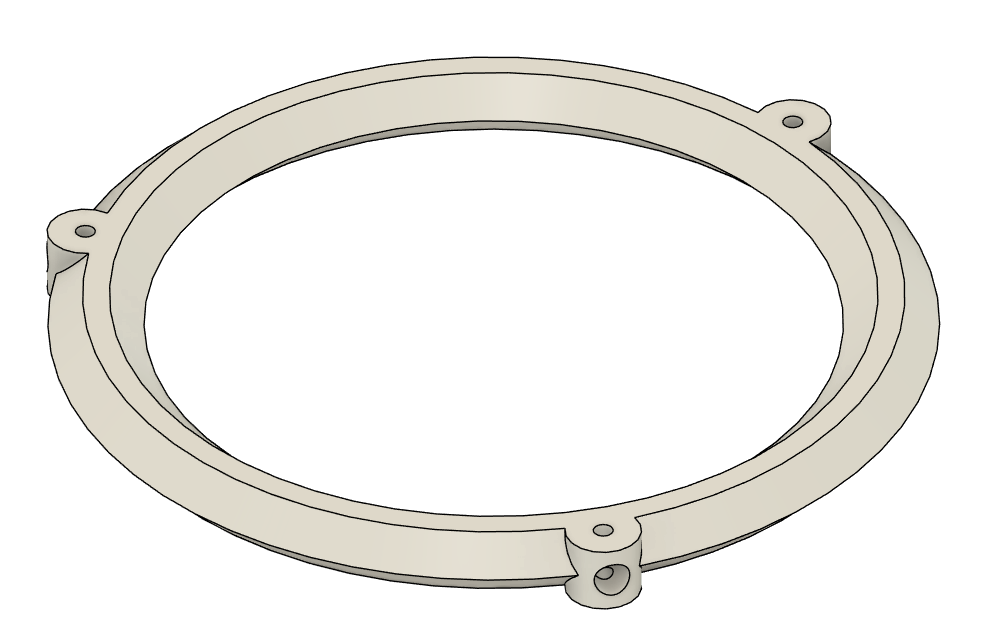
\includegraphics[width=\textwidth]{constraint_view}
        \caption{General view}
        \label{fig:cons_view}
    \end{subfigure}
    \begin{subfigure}[t]{0.6\textwidth}
        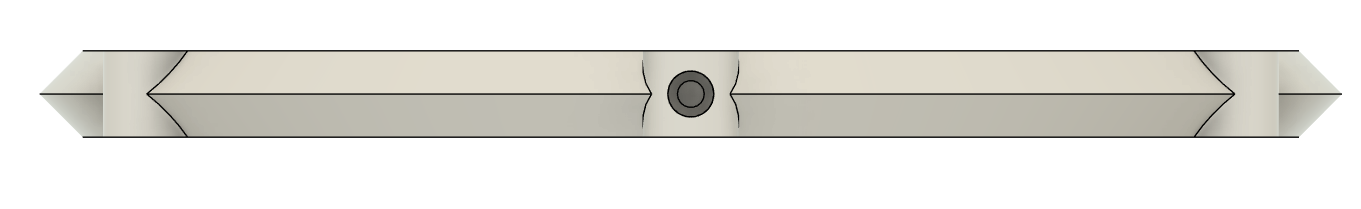
\includegraphics[width=\textwidth]{constraint_frontal_view}
        \caption{Lateral view}
        \label{fig:cons_front_view}
    \end{subfigure}
    \caption{Ring constraint}
    \label{ring_constraint}
\end{figure}


\begin{figure}
    \centering
    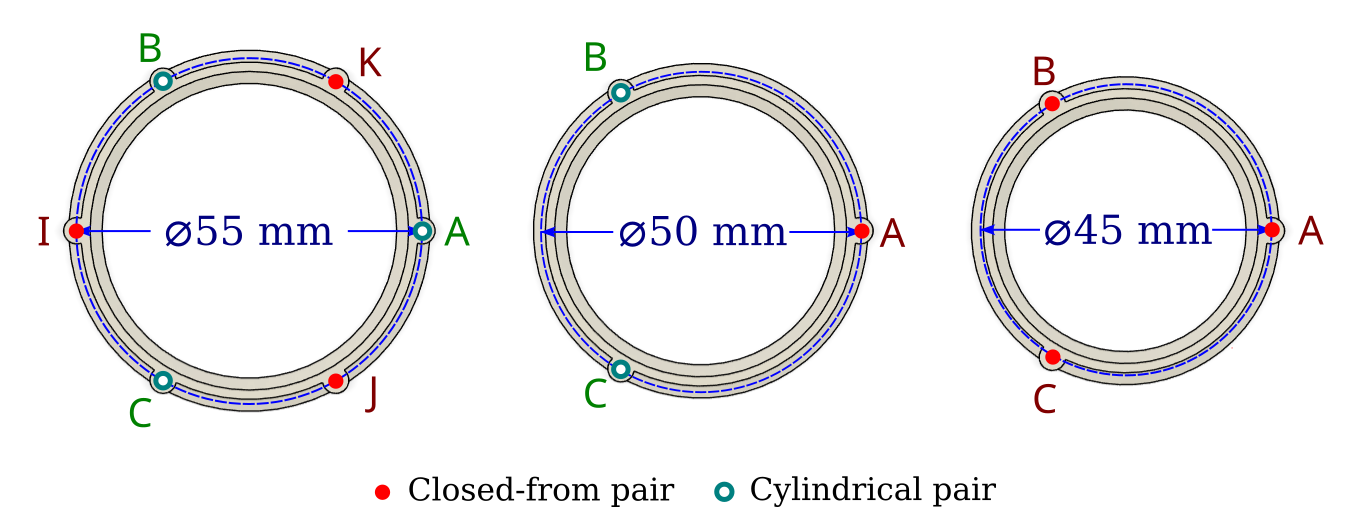
\includegraphics[width=0.9\textwidth]{constraint_sizes}
    \caption{Ring constraint sizes}
    \label{fig:cons_sizes}
    \caption*{In \textit{blue}, the diameters of the circumferences enclosing the rods are shown. The rods are labeled \textit{A}, \textit{B}, \textit{C}, \textit{I}, \textit{J}, \textit{K}. The \textit{green} open circle indicates a cylindrical pair constraint between the ring and the rod, while the \textit{red} indicates a closed-form pair constraint involving both.}
\end{figure}

\begin{figure}
    \centering
    \begin{subfigure}[t]{0.45\textwidth}
        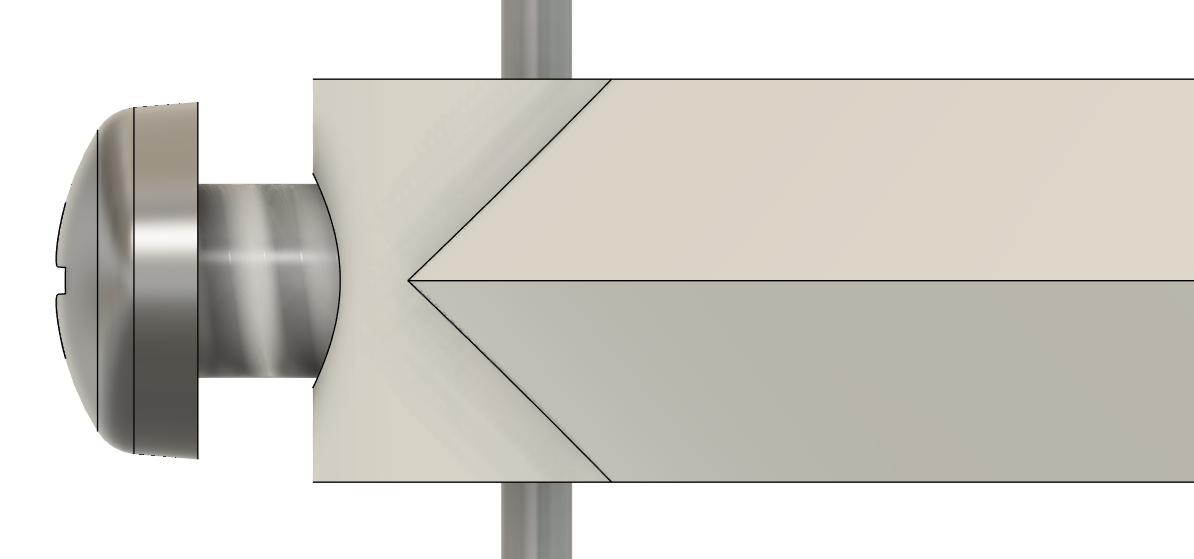
\includegraphics[width=\textwidth]{constraint_screw_rod}
        \caption{Physical closed-form pair constraint}
        \label{fig:cons_physical}
    \end{subfigure}
    \begin{subfigure}[t]{0.45\textwidth}
        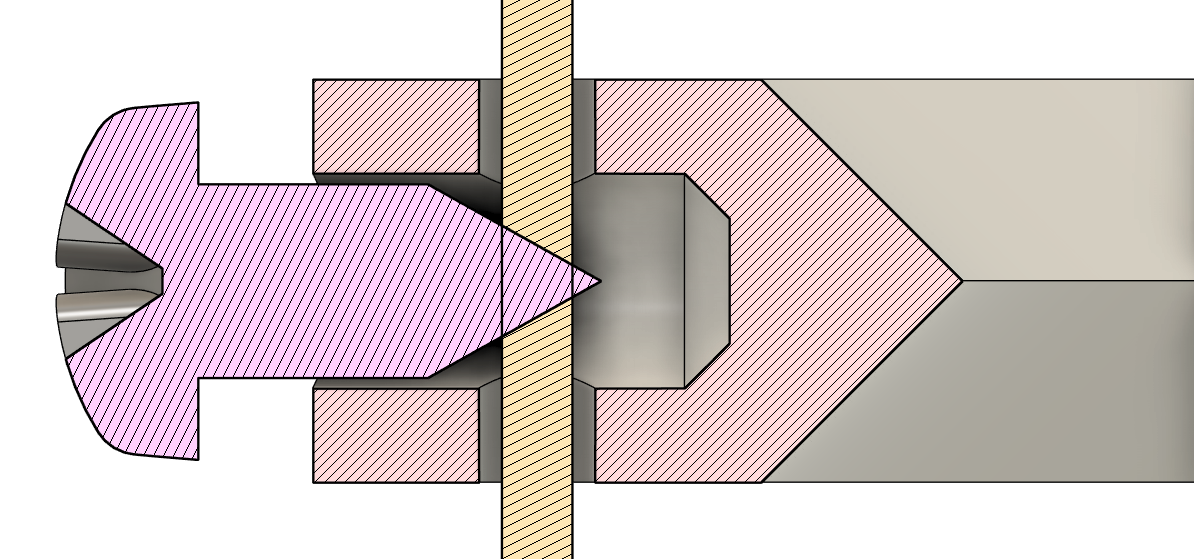
\includegraphics[width=\textwidth]{constraint_section_view}
        \caption{Section view of closed-form pair constraint}
        \label{fig:cons_physical_section}
    \end{subfigure}
    \caption{Closed-form pair constraint}
    \label{closed_constraint}
\end{figure}
